% ORGANIZACIÓN DE COMPUTADORAS
% SEGUNDO CUATRIMESTRE 2017
% PRIMER EXAMEN PARCIAL

\documentclass[12pt,a4paper]{article}
\usepackage[spanish]{babel}
\selectlanguage{spanish}
\usepackage[utf8]{inputenc}

\usepackage{graphicx}
\usepackage{multirow}
\usepackage{xcolor}
\usepackage{fancyhdr}
\renewcommand{\headrulewidth}{0pt}

\setlength{\textwidth}{170mm}
\setlength{\oddsidemargin}{-5.4mm}
\setlength{\evensidemargin}{-5.4mm}
\setlength{\textheight}{247mm}
\setlength{\topmargin}{-15.4mm}
\setlength{\headheight}{11mm}
\setlength{\headsep}{2mm}

% CARPETA CON IMAGENES DE ENCABEZADO
\graphicspath{{estilo/}}

% DEFINICIÓN DE COMANDOS

\newcommand{\setyear}[1]{\year=#1}
\newcommand{\universidad}{Universidad Nacional del Sur}
\newcommand{\departamento}{Departamento de Ciencias e Ingeniería de la Computación}
\newcommand{\materia}{Organización de computadoras}
\newcommand{\cuatrimestre}{Segundo}

\newcommand{\RISC}{\textsc{risc}}
\newcommand{\CISC}{\textsc{cisc}}
\newcommand{\OCUNS}{\textsc{ocuns}}
\newcommand{\PC}{\textsf{PC}}
\newcommand{\SP}{\textsf{SP}}

% ENCABEZADO GENERAL
% DeptoLogo - Departamento - Universidad - Cuatrimestre - Año - UniLogo
\newcommand{\header}{
	\begin{center}
		\begin{tabular}{lcl}
		\multirow{4}{*}
		{\smash{$\vcenter{\hbox{
\includegraphics[width=.78in]{DeptoLogo}}}$}} & {\Large\textsc{\materia}} &  
		\multirow{4}{*}
		{\smash{$\vcenter{\hbox{
\includegraphics[width=.88in]{UniLogo}}}$}} \\
		         & \departamento & \\
		         & \universidad & \\
		         & \textbf{\cuatrimestre\ Cuatrimestre de \number\year} & \\
		\end{tabular}\\[2em]
	\end{center}
}

% ENCABEZADO EDITABLE%
% Uso: \Titulo{Primer texto negrita}{Segundo texto normal}
% header + Texto 1 + Texto 2
\newcommand{\Titulo}[2]{ 
	\begin{center}
		\header
		 \textbf{#1} \\ #2 \\[4pt]
	\end{center}
}

% ENCABEZADO PRÁCTICOS CON NUMEROS
% Uso: \TPnumero{Número de Práctico}{Título de Práctico}
% header + Trabajo Práctico Nº X + Titulo de Práctico
\newcommand{\TPnumero}[2]{ 
	\begin{center}
		\header
        Trabajo Práctico N$^{\circ}$ #1 \\ \textbf{#2} \\[4pt]
    \end{center}
}

% ENCABEZADO PRÁCTICOS CON LETRAS
% Uso: \TPletra{Letra de Práctico}{Título de Práctico}
% header + Trabajo Práctico 'X' + Titulo de Práctico
\newcommand{\TPletra}[2]{ 
	\begin{center}
		\header
		Trabajo Práctico #1 \\ \textbf{#2} \\[4pt]
	\end{center}
}

% ENCABEZADO PRÁCTICOS PROGRAMACIÓN CON NUMEROS
% Uso: \TPPnumero{Número de Práctico}{Título de Práctico}
% header + Trabajo Práctico de Programación Nº X + Titulo de Práctico
\newcommand{\TPPnumero}[2]{ 
	\begin{center}
		\header
		Trabajo Práctico de Programación N$^{\circ}$ #1 \\ \textbf{#2} \\[4pt]
	\end{center}
}

% ENCABEZADO PRÁCTICOS PROGRAMACIÓN CON LETRAS
% Uso: \TPPletra{Letra de Práctico}{Título de Práctico}
% header + Trabajo Práctico de Programación 'X' + Titulo de Práctico
\newcommand{\TPPletra}[2]{ 
	\begin{center}
		\header
		Trabajo Práctico de Programación #1 \\ \textbf{#2} \\[4pt]
	\end{center}
}

% ENCABEZADO PROYECTO CON NÚMERO
% Uso: \PRnumero{Número de Proyecto}{Título de Proyecto}
% header + Proyecto Nº X + Titulo de Proyecto
\newcommand{\PRnumero}[2]{
	\begin{center}
		\header
		Proyecto N$^{\circ}$ #1 \\ \textbf{#2} \\[4pt]
	\end{center}
}

\begin{document}

\Examen{Primer Examen Parcial}

\begin{centering}
\emph{Apague cualquier dispositivo electrónico en su poder y manténgalo guardado. No puede utilizar auriculares, ni calculadora. Lea todo el ejercicio antes de comenzar a desarrollarlo.}	
\end{centering}

\PEjercicio{1}Dado el número \textbf{decimal} $-298.5625$ llevar adelante los siguientes cambios de base:
\begin{enumerate}[a)]
	\item Convertirlo a \textbf{octal}, empleando el método de la \textbf{división} tanto para la parte entera como para la parte fraccionaria, expresando el resultado en \textbf{complemento a la base}, con 4 dígitos octales para la parte entera y 6 para la parte fraccionaria.

	\item Convertirlo a \textbf{binario} utilizando el método de la \textbf{multiplicación} tanto para la parte entera como para la parte fraccionaria, expresando el resultado en \textbf{complemento a la base disminuida}, con 12 bits para la parte entera y 6 bits para la parte fraccionaria.
\end{enumerate}

\PEjercicio{2}Considerando los números {\textbf{decimales}} $X = 1537$ e $Y = 2559$, llevar adelante las siguientes operaciones, indicando claramente el resultado obtenido y la existencia o no de \emph{overflow}:
\begin{enumerate}[a)]
	\item Calcular $- X - Y$, trabajando en \textbf{hexadecimal} en \textbf{complemento a la base}, con una precisión de cuatro dígitos (incluido el signo).
	\item Calcular $ X + Y $, trabajando en \textbf{hexadecimal} en \textbf{complemento a la base disminuida}, con una precisión de cuatro dígitos (incluido el signo).
	\item Calcular $X - Y$, haciendo uso de un hardware que opera en una codificación \textbf{BCD Exceso-3} y \textbf{complemento a la base}, con una precisión de cinco dígitos (incluido el signo), indicando claramente qué operación se está realizando en cada uno de los pasos intermedios.
\end{enumerate}

\PEjercicio{3} Considerando el Código Cíclico Redundante (CRC):
\begin{enumerate}[a)]
	\item Construir el mensaje $T(x)$ a transmitir asociado al mensaje de datos
	$M(x) = 110\,1011\,1011$ empleando el polinomio generador $G(x) = x^4 + x + 1$.

	\item Suponiendo que durante la transmisión el mensaje $T(x)$ es modificado con un error $E(x)$ de tal forma que el receptor recibe el mensaje $T'(x) = 110\,\, 0011\,0011\,1011$, determinar cómo opera el mecanismo de detección de errores y cuál es la conclusión que se alcanza.

	\item Comparando el mensaje transmitido $T(x)$ y el mensaje recibido $T'(x)$, ¿cuál es el desarrollo del polinomio de error $E(x)$? Sabiendo cuál fue el error exacto que existió, ¿cuál es la longitud de la ráfaga en error? y ¿a qué conclusión se puede arribar?
\end{enumerate}

\PEjercicio{4} Considerando el código Hamming mínima distancia 4 (Hamming extendido), empleando paridad par y estando la secuencia ordenada de izquierda a derecha:
\begin{enumerate}[a)]

	\item Calcular los bits de código asociados al dato $0110\,1011$ y armar el codeword correspondiente que integra el dato y los bits calculados. ¿Cuántos bits de código se tienen que completar? Justifique su respuesta. 

	\item Considerando que el receptor recibe el codeword $1\,0111\,1011\,0110$ que contiene los bits de dato y de código $C_i$. Recalcular los bits de código y determinar cuál es el síndrome.

	\item Determinar cómo trabaja el mecanismo de detección/corrección ante una política $d=2$, $c=1$, con los resultados obtenidos en el inciso b).

	\item Determinar cómo trabaja el mecanismo de detección/corrección ante una política $d=3$, $c=0$, si el síndrome fuera $1110$.

	\item Determinar cómo trabaja el mecanismo de detección/corrección ante una política $d=2$, $c=1$, si el síndrome fuera $0000$.

%	\item Determinar cómo trabaja el mecanismo de detección/corrección antes una política $d=3$, $c=0$ cuando al recalcular los bits de código de un codeword recibido se obtiene síndrome $0000$.

\end{enumerate}

\PEjercicio{5} Dada la definición para \texttt{TCadena}, implementar en \textbf{lenguaje C}:
\begin{enumerate}[a)]
	\item Una función \texttt{int es\_palindroma(TCadena cad)} que dada una cadena de caracteres \texttt{cad}, retorne 1 si \texttt{cad} es \textit{palíndroma}, y cero en caso contrario. Una cadena de caracteres se dice \textit{palíndroma}, si se lee de igual forma de izquierda a derecha que de derecha a izquierda. Ejemplo: ``anana'' y ``neuquen'', son cadenas \textit{palíndromas}.
	\item Una función \texttt{TCadena[] clonar (TCadena[] arr, int long)}, que dado un arreglo de cadenas de caracteres \texttt{arr} de longitud \texttt{long}, retorne un nuevo arreglo de cadenas de igual longitud que \texttt{arr}, pero que contenga la \textit{clonación} de aquellas cadenas en \texttt{arr} que son \textit{palíndromas}. Para esto, contemplar el uso de la función definida en el inciso anterior, así como un correcto uso de la función \texttt{malloc} para reservar memoria a la hora de clonar las cadenas.
\end{enumerate}
Dado un \textit{Arreglo A}, la función \texttt{clonar()} retornará un nuevo \textit{Arreglo B}, tal como se indica en la siguiente figura:\\
\begin{centering}
	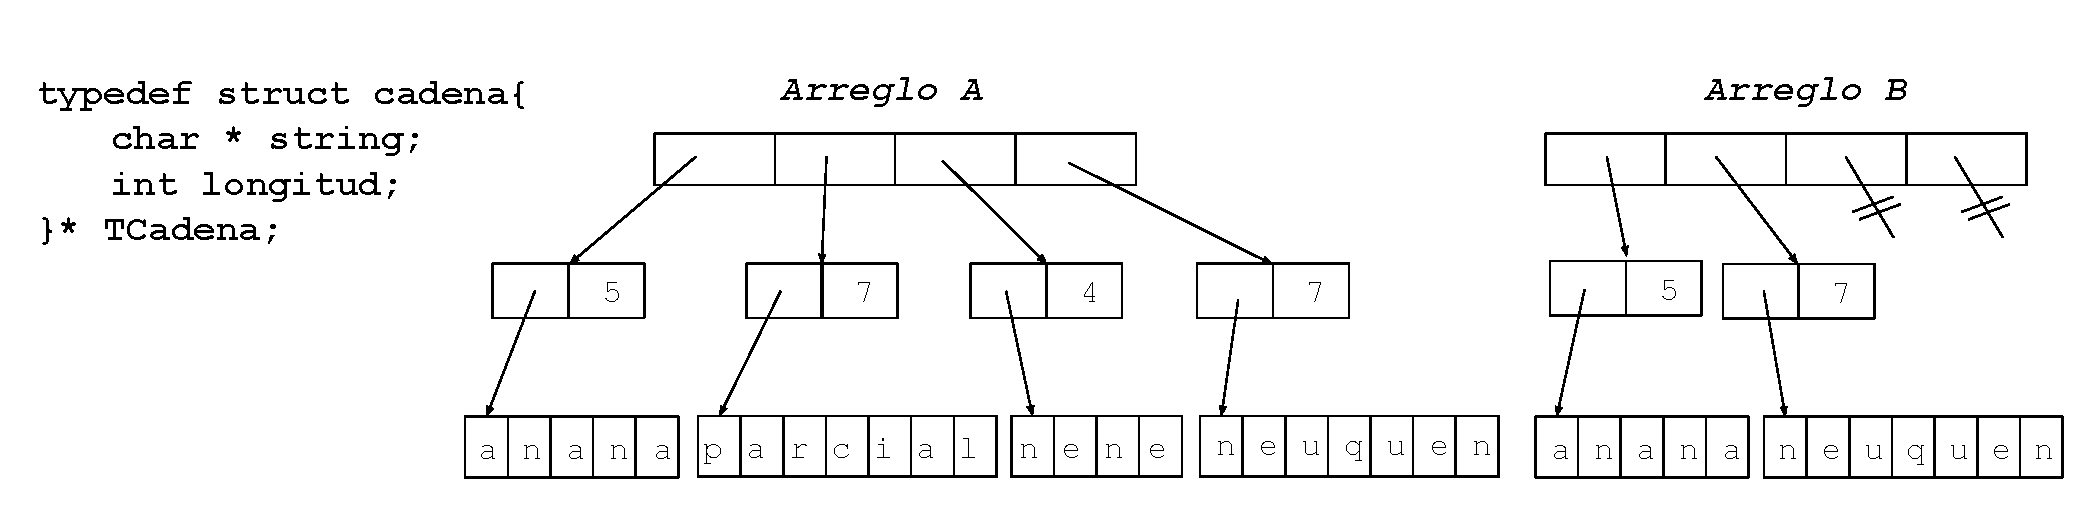
\includegraphics[height=0.2\textheight, width=1.05\textwidth]{Ejercicio_5.pdf} 
\end{centering}
\end{document}

